% References:
% https://nlp.stanford.edu/software/stanford-dependencies.shtml
% https://downloads.cs.stanford.edu/nlp/software/dependencies_manual.pdf
% https://www.ling.upenn.edu/courses/Fall_2003/ling001/penn_treebank_pos.html
% https://catalog.ldc.upenn.edu/docs/LDC95T7/cl93.html

\begin{figure}[!tb]
\centerline{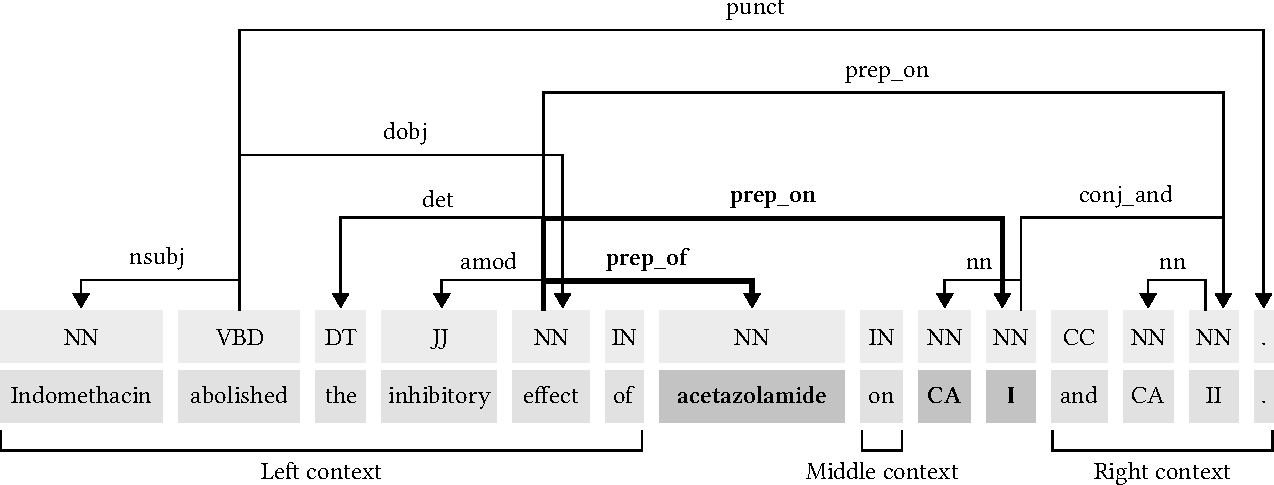
\includegraphics[width=\textwidth]{img/chemprot-sdp/v2/img.pdf}}
\caption[Example illustrating the dependency parsing structure of a sentence.]%
{Example illustrating the dependency parsing structure of a sentence from the ChemProt training dataset (PMID 8667211). In this example, we considered the relation between the `acetazolamide' chemical mention and the `CA I' protein mention. The shortest dependency path is highlighted in bold. Penn Treebank part-of-speech tags \parencite{marcus1993a} used in this example: coordinating conjunction (CC); determiner (DT); preposition or subordinating conjunction (IN); adjective (JJ); noun, singular or mass (NN); verb, past tense (VBD); sentence final punctuation (.). Stanford dependencies \parencite{marneffe2016a} used in this example: adjectival modifier (amod); conjunction and (conj\_and); determiner (det); direct object (dobj); noun compound modifier (nn); nominal subject (nsubj); prepositional modifier of (prep\_of); prepositional modifier on (prep\_on); punctuation (punct).}
\label{fig:chemprot-sdp}
\end{figure}
